\documentclass[a4paper,11pt]{article} 

% \documentclass[a4paper,11pt]{book} 

\usepackage[T1]{fontenc}
\usepackage[utf8]{inputenc}
\usepackage[spanish]{babel}

\usepackage{graphicx}

\usepackage{colortbl}
\usepackage{color}

\usepackage{hyperref}

\usepackage[margin=1in]{geometry}
\pagestyle{plain}

%\usepackage{fancyhdr} 
%\usepackage{lastpage}
%\usepackage{float} 
%\floatstyle{boxed} 
%\restylefloat{figure} 
%\pagestyle{fancy}

\setcounter{secnumdepth}{5}
\setcounter{tocdepth}{6}

\definecolor{orange}{RGB}{0,0,255}
\setcounter{secnumdepth}{5}
\setcounter{tocdepth}{5}
%\title{\textcolor{orange}{Guia Practica Instalación de MinSoc}}
%\author{Gomez,Roberto Pablo - Lovaisa Michelini, Valeria  \\ Universidad Tecnológica Nacional \\ CUDAR }

\begin{document}

%\lhead{\includegraphics[width=1\textwidth]{encab.png}}
%\lfoot{{\includegraphics[width=1\textwidth]{pie.png}}}
%\rfoot{\thepage}

%\maketitle 
%\newpage

\tableofcontents


\newpage

\section{\textcolor{orange}{Introducción}}
\subsection{\textcolor{orange}{Descripción General}}
Descripción por arriba del trabajo. por ejemplo la industria dispone de herramientas que nosotros usamos para un fin determinado.

\subsection{\textcolor{orange}{Objetivos}}
\subsubsection{\textcolor{orange}{Objetivo General}}

Implementar un system on chip OpenSource con un microprocesador embebido Soft-core que soporte un sistema operativo libre , con la finalidad de entregar un sitema integral FPGA-SoC-Sistema Operativo completamente funcional y bajo licencia GPL v2.

\subsubsection{\textcolor{orange}{Objetivo Específico}}
\begin{itemize}
\item Seleccionar, analizar y determinar un microprocesador Sof-Core.
\item Establecer un system on chip Open Source donde poder implementar un Soft-Core.
\item Determinar sistemas operativo con licencia GPL v2 que tengan las prestaciones funcionales adecuadas.
%\item Evaluar, seleccionar una plataforma objetivo un entorno de trabajo  las prestaciones de los Kit de desarrollos con FPGA disponibles en el área de trabajo.
%\item Evaluar, seleccionar y validar las prestaciones de los Kit de desarrollos con FPGA disponibles en el área de trabajo.
%\item Analizar un soft-core que me de las prestaciones funcionales que cumplan de  los requerimientos 
%\ Obtener  completamente funcional sobre un kit de desarrollo XILINX XtremeDSP Starter Platform Spartan 3A DSP 1800.
%\item Implementar un Sistema Operativo eCos sobre un SoC de codigo abierto en el Kit de desarrollo XILINX XtremeDSP Starter Platform Spartan 3A DSP 1800.
%\item Implementar un Sistema Operativo Linux sobre un SoC de codigo abierto en el Kit de desarrollo XILINX XtremeDSP Starter Platform Spartan 3A DSP 1800 .
%\item Probar el adecuado funcionamiento de el sistema global que tenga las  prestaciones funcional  
%tradicionales de diseño
\end{itemize}

\subsection{\textcolor{orange}{Motivación}}

Existe un grupo de cores Sof-Core de código abierto que no están limitados por la tecnología. Los cores destacados de microprocesadores de 32 bits, son los procesadores SPARC LEON OpenRISC 1200 , y el core de LatticeMico32. Usar cores de  codigo abierto,  va unido a una serie de conceptos como:
 \begin {itemize}
\item Flexibilidad. Si el codigo fuente está disponible, los desarrolladores pueden modificar el codigo de acuerdo a sus necesidades.Adémas, se produce un flujo constante de ideas que mejora la calidad del codigo.
\item Fiabilidad y seguridad. Con muchos programadores a la vez escrutando el mismo trabajo, los errores se detectan y corrigen antes, por lo que el producto resultante es mas fiable y eficaz que el comercial.
\item Rapidez de desarrollo. Las actualizaciones y ajustes se realizan a través de una comunicación constante vía Internet.
\item Relación con el usuario. El programador se acerca mucho mas a las necesidades reales de su cliente, y puede crear un producto especifíco para él
 \end {itemize}
 
Obtener un sistema integral de código abierto en donde se tiene código HDL, assembler y C disponible para adaptarse de acuerdo a los requerimientos del proyecto. Ademas de la de la capacidad de migrar de una plataforma a otra. Logrando menor dependencia entre el código fuente y la plataforma objetivo. 
La portabilidad del codigo abierto nos permite implementarlo sobre una ASICs (Application-specific integrated circuit) o con modificaciones menores en cualquier FPGA (Field Programmable Gate Array) de Xilinx, Altera, Lattice, etc. 

Estos tres de los más grandes proveedores de FPGA , Xilinx , Altera y Lattice , ofrecen sus propios micro core RISC de 32bits los dos mayores proveedores de dispositivos FPGA , Altera y Xilinx , proporcionan el micro core Nios y Microblaze, respectivamente. Son micro cores  en donde el codigo fuente RTL no se encuera disponible y solo pueden ser implementados en sus respectivas FPGA.
 
Una de principales ventajas de usar plataformas con FPGA, es que son flexibles asi que pueden adaptarse a diferentes funciones. Los componentes de hardware ofrecen mucho mayor rendimiento que el software equivalente. Los cuellos de botella de procesamiento del sistema pueden identificarse y sustituirse por hardware, de manera que se evita la costosa optimizan del software.

\subsection{\textcolor{orange}{Importancia del Problema}}

En el diseño del sistema embebido se usan diferentes procesos depende del tipo de sistema, el hardware disponible y la organización que desarrolle el sistema. Una de las actividades principales en un proceso de diseño de software es la elección del hardware y del sistema operativo que se efectúa antes del comienzo del software. Ante tal situación , se debe diseñar el software par considerar las restricciones impuestas por las capacidades del hardware.
Los efectos que influyen dichas elecciones comprenden restricciones de de temporización sobre el sistema, limitación en la energía disponible, experiencia del equipo de desarrollo y limites en el costos del sistema entregable.
 
Se está explorando una linea donde se busca dar al diseñador del sistema embebido una solución flexible en la primera etapa de la elección de plataforma. Donde a través del análisis de diferentes plataformas de desarrollo OpenSource y privativas pueda elegir la mejor opción para el tipo de sistema a desarrollar y requerimientos de proceso. 
 
Una vez que se ha elegido la plataforma de ejecucion para el sistema, se ha diseñado una arquitectura de proceso y se a determinado una políticas de planeación, es necesario comprobar que el sistema cumplirá sus con sus requerimientos.

\subsection{\textcolor{orange}{Alcance del Estudio}}

Debido al plazo estipulado para el desarrollo del proyecto, el mismo involucra tres etapas: 

 \begin {itemize}
\item Especificación y Análisis de requerimientos.
\item Implementación.
\item Testing.
 \end {itemize}


%de donde hasta donde vamos a ir
%primero elegimos un micro después lo embebemos en un soc y después le metimos un sistema operativo
\subsection{\textcolor{orange}{Modelo de Desarrollo}}


El modelo de desarrollo a utilizar es el Modelo en Espiral tipificado por Ian Sommerville [2] . El modelo en espiral de ingeniería de software, mostrado en la Ilustración 1, fue originalmente propuesto por Boehm en año 1988, en su artículo A Spiral Model of Software Development and Enhancement. Propuso un marco del proceso de software dirigido por el riesgo. Aquí, el proceso de software se representa como una es espiral, cada ciclo en la espiral representa una fase del proceso de software. Por ende el, ciclo más interno puede relacionarse con la factibilidad del sistema, el siguiente ciclo con la definición de requerimientos, el siguiente ciclo al diseño del sistema, y así sucesivamente.
Cada ciclo del espiral se divide en 4 sectores:
 
\begin {itemize}
\item Establecimiento de objetivo  Se definen objetivos específicos para dicha fase del proyecto. Se identifican restricciones en el proceso y el producto, y se traza un plan detallado de gestión. Se identifican los riesgos del proyecto. Dependiendo de estos riegos, se planean estrategias alternativas
\item Validación y reducción del riesgo  En cada uno de los riesgos identificados del proyecto, se realiza un análisis minucioso. Se dan acciones para reducir el riesgo.
\item Desarrollo y validación  Despues de una evaluacion del riesgo, se elige un modelo de desarrollo para el sistema.
\item Planeción  El proyecto se revisa y se toma una decisión sobre si hay que continuar con otro ciclo de la espiral. Si se opta por continuar, se trazan los planes para la siguente fase del proyecto.
 \end {itemize}mn

Como característica principal de esta metodología es que posee una consideración explícita del riesgo. Informalmente, el riesgo significa sencillamente que algo puede ir mal. Los riegos originan problemas en el proyecto, como los de confección de agendas y excesos en los costos; por lo tanto, la disminución de riegos es una actividad sumamente importante en la gestión del proyecto.
Un ciclo en la espiral comienza con la elaboración de objetivos, como el rendimiento y la funcionalidad. Entonces se enumeran formas alternativas de alcanzar estos objetivos y las restricciones impuestas en cada una de ellas. Cada alternativa se evalúa contra cada objetivo y se identifican las fuentes de riegos del proyecto. El siguiente paso es resolver estos riesgos mediante actividades de recopilación de información como la de detallar más el análisis, la construcción de prototipos y la simulación. Una vez que se han evaluado los riesgos se llevará a cabo cierto desarrollo, seguido de una actividad de planificación para la siguiente fase del proceso.

\subsection{\textcolor{orange}{Metodología}}

Considerando que el objetivo planteado es un desarrollo que se realiza por primera vez, se aplicará un desarrollo experimental y de simulación. La falta de documentación al respecto y al ser un desarrollo de vanguardia son factores que acentúan en esta decisión. Sumado a lo anteriormente dicho, en el laboratorio donde se desarrolla este proyecto no existen antecedentes de trabajos similares.
 
Se utilizó como metodología en este desarrollo el modelo de componentes, donde se define estándares para la implementación, documentación y el despliegue de componentes. 


%\section{\textcolor{orange}{Perspectiva Historica}}
%	\subsection{\textcolor{orange}{El Comienzo de los Microprocesadores}}
%	\subsection{\textcolor{orange}{FPGAs y Microsprocesadores Soft-Core}}
%	\subsection{\textcolor{orange}{Software OpenSource y Libre}}
 %%%%%%%%%%%%%%%%%%%%%%%%%%%%%%%%%%%%%%%%%%%%%%%%%%CAPITULO 2%%%%%%%%%%%%%%%%%%%%%%%%%%%%%%%%%%%%%%%%%%%%%%%%%%%%%%%%%%%%%%%%

\section{\textcolor{orange}{FPGA y microprocesadores Soft-Core}}%julius
	\subsection{\textcolor{orange}{FPGAs}}

La fabricación de dispositivos semiconductores es un proceso complicado de plazos largos y costoso. Esto lleva a que los diseños destinados para la  implementacion en chip de silicio tengan poco oportunidad de ser prototipados antes de que comience la producción en grandes volúmenes. Esto supone una gran importancia  en las faces de prueba y verificación de un diseño antes de ser fabricado.

Basándose en la predicción de la ley de Moore donde expresa que aproximadamente cada dos años se duplica el número de transistores en un circuito integrado\cite{Etiqueta01}, Ross Freeman postulo que los transistores serian menos costoso cada año, haciendo asequible la fabricación de chips programables personalizables \cite{Etiqueta03}.
La compañía Xilinx, ofreció su primer chip en 1984 , que contiene arrays celdas lógicas (LCAs) , programables por el usuario en casi cualquier configuración que quisieran. Estos se conocen como Field Programmable Gate Array (FPGAs) .

Las FPGAs desempeñan un papel dual, uno como objetivo final de ejecución en un diseño y otro papel como prototipo para la implmentacion definitiva de un diseño. Su capacidad de reconfigurar el diseño parcial o totalmente para su actualización o corrección de errores tiene un costo relativamente bajo a diferencia del prototipado sobre ASICs.
Actualmente las FPGA cuentan con una gran cantidad de recursos disponibles (Compuertas lógicas , Bloques de RAM) para implementar diseños digitales complejos.

Una desventaja de las FPGA  es debido a la naturaleza inherente de las arquitecturas de FPGA, los diseños implementados en FPGA comparados con una ASICs en general tienen mas area, menos porformance y consumen mas energía.

		\subsubsection{\textcolor{orange}{Arquitectura}}	

Los componentes de una \textit{FPGA} se pueden dividir en cinco grupos:

\begin {itemize}
\item  Bloques lógicos configurables y \textit{Lookup Tables}.
\item  Bloques de entrada y salida.
\item  Bloques multiplicadores
\item  Bloques Manejadores de Clock Digitales.
 \end {itemize}

\begin{figure}[h!]
 \begin{center}
 % 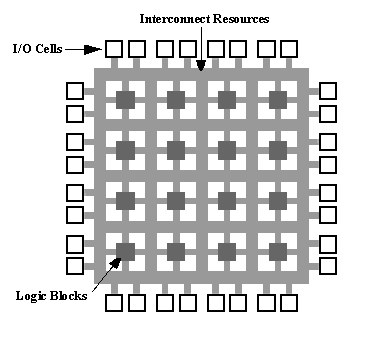
\includegraphics[width=0.5\textwidth,keepaspectratio=true]{./images/fpga1a.gif}
  \caption{Componentes de una FPGA}
  \label{fig:esquema}
 \end{center}
\end{figure}

		\subsubsection{\textcolor{orange}{Bloques Lógicos Configurables y Lookup Tables}}
Todas las \textit{FPGA} se basan en arrays de pequeños elementos de lógica digital. Los problemas de lógica digital se descomponen en circuitos lógicos que puedan ser mapeados a uno o más de estas “celdas lógicas” a través de un proceso llamado “technology mapping".

Cada bloque de logica configurable varia de acuerdo a su fabricante, en el caso de Xilinx tienen el nombre Logic cell (LC) contiene una 4 input LUT, un multiplexor y un registro. Se puede configurar la polaridad del clock, el clock enable y la señal de reset.


\begin{figure}[h!]
 \begin{center}
 %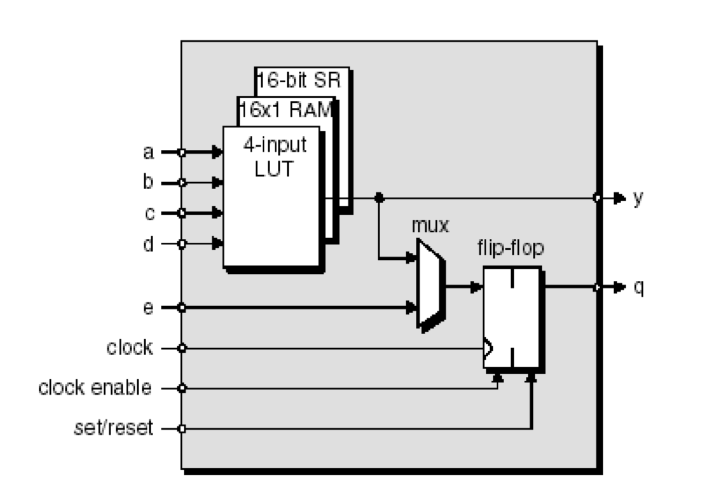
\includegraphics[width=0.5\textwidth,keepaspectratio=true]{./images/celda}
  \caption{Componentes de una FPGA}
  \label{fig:esquema}
 \end{center}
\end{figure}

También se encuentran las Lookup Tables, que son elementos lógicos que están compuestos de al menos un registro programable (flip\-flop) y alguna lógica de entrada, que usualmente está implementada como una lookup table de n entradas, donde n es 5 o menos. Estas LUTs son capaces de implementar cualquier función combinacional de sus entradas.

		\subsubsection{\textcolor{orange}{Bloques de Entrada y Salida de propósito general }}

Las FPGAs poseen pines TTL, CMOS, PCI, LVDS y muchos otros que les permiten hacer de interface y convertir muchas tecnologías diferentes. Las FPGAs tienen bloques de I/O dedicados para clocks y resets globales. También incluyen PLL y esquemas para el manejo de clocks permitiendo múltiples dominios del mismo.

Las FPGAs actuales tienen impedancias de I/O configurables,  permiten el uso de resistencias internas terminales cuyos valores pueden ser configurados por el usuario. 


		\subsubsection{\textcolor{orange}{Bloques de Memoria}}

Las FPGAs actuales incorporan memorias on-chip, tales como las SRAM. Estas memorias pueden ser accedidas en forma jerárquica, desde la memoria local de cada celda a la memoria global de los bloques compartidos de memoria. Si bien esto no hace a la esencia de la FPGA, todas hoy en día poseen estos bloques para dar solución al impacto que conlleva utilizar una memoria externa al chip, mayormente soluciona los problemas de latencia.

		\subsubsection{\textcolor{orange}{Multiplicadores}}
Algunas funciones como los multiplicadores son muy lentos si se implementan mediante la conexión de un gran numero de bloques lógicos. Por eso muchas FPGAs incorporan bloques multiplicadores hardware. Estos bloques se encuentran muy cerca de los bloques de RAM embebidos. 
\subsubsection{\textcolor{orange}{Manejadores de Clock Digitales}}
 Se llama clock tree porque la señal de clock principal es ramificada para que alcance a todos los flip-flops.Esta estructura es así para asegurarse que todos los flip flop estén lo mas cerca posible del clock y evitar el problema del skew.El clock tree es implementado usando canales separados de los de propósito general para interconectar los bloques.

		\subsection{\textcolor{orange}{Microprocesadores Soft-Core }}

El avance en la en la tecnología de fabricación de VLSI (Very Large Scale Integratio) a medida que se agregaron más y más transistores,y en consecuencia más y más funciones fueron integradas en un mismo chip, por lo tanto también las capacidades en FPGAs. Grandes diseños de sistemas digitales que fueron sólo para ser implementado como ASICs, luego tuvieron la opción de ser ejecutados en FPGA.

El microprocesador, ya sea como un componente discreto o  como parte de otra lógica en el mismo chip, es una candidato  para ser  implementado en FPGA. Esto introdujo un mayor potencial para la exploración del espacio de diseño haciendo que la logica de computo especifica sea implemetada junto con un microprocesador estándar %\cita{estiqueta20}
		
	\subsubsection{\textcolor{orange}{ IP-Core}}

El diseños de circuitos digitales se dividen normalmente en bloques funcionales, que se refiere como módulos, o \textit{cores}. Un \textit{core} estara formado por sub-bloques que ayudan a poner en práctica su funcionalidad. Los \textit{cores} pueden variar en tamaño hasta el tamaño total de un microprocesador. Un \textit{core} puede ocupar una FPGA entera al ser implementado, mientras que sólo se crea una instancia entre otros en una FPGA más grande o en un ASIC. Los \textit{núcleos} se describen generalmente utilizando un lenguaje de descripción de hardware (HDL) en un nivel de abstracción conocida como registro nivel de transferencia (RTL).

El proceso de tomar la descripción RTL de un diseño y convertirlo en un lista de primitivas o puertas lógicas y las conexiones entre ellos, dejando luego que la  implementación se realice en una tecnología de destino, se conoce como\textit{síntesis}. Analogamente a la compilación de software - que se tiene un programa en un lenguaje de alto nivel, como C, y  es convertido a codigo maquina. 

El resultado de la síntesis, conocida como una \textit{netlist}, está en un nivel de abstracción denominado nivel de la puerta.En pocas palabras, es esta lista de conexiones que se utiliza para su posterior procesamiento en una configuración para FPGA o en un diseño para ASIC.

Los cores pueden ser diseñados por una persona o entidad, los desarrolladores de \textit{cores} y licenciatarios varían en tamaño desde particulares a empresas de miles de millones de dólares. El producto, en este caso se conoce como un \textit{IP core  Intellectual Property Core} el diseño es la propiedad intelectual de los desarrolladores de terceros y la derecho a usarla recibe la licencia del cliente. La \textit{Intellectual Property IP} varia  de  acuerdo a las licencia.

			\paragraph{\textcolor{orange}{ Tipos de IP-Core}}
hard soft y intermedios
%El producto , en este caso se conoce como un núcleo IP (propiedad intelectual a menudocore) en el sentido de que el diseño es la propiedad intelectual de los desarrolladores de terceros y le da derecho a usarlo  recibe la licencia del cliente. Se utilizan los términos IP y el núcleo indistintamente y en combinación para significar la misma cosa .IP puede ser en una variedad de formas cuando licencia . Cuando está en la forma de sintetizable RTL entonces el IP se conoce como un núcleo blando . Si se trata de una forma menos abstraído forma , tal como un formato de un mensaje - diseño listo lista de conexiones o para la fabricación, que se conoce como IP núcleo duro .

\subsection{System on Chip}

La innovación continua en la tecnología de fabricación de semiconductores, ha visto al
disponible "real estate" en los chips de aumento en línea con la predicción de 1965 por Gordon E. Moore. La capacidad de los ingenieros de diseño digital para hacer uso de estos transistores adicionales no ha seguido el ritmo de este incremento en la capacidad de fabricación (21). El tiempo para las necesidades del mercado de estos diseños cadam vez más complejos ha permanecido estático, si no apretado.

Esto ha llevado a la aparición de la industria de núcleo IP compuesta de las empresas especializadas en el desarrollo y concesión de licencias IP a las personas la construcción de sistemas de FPGA o ASIC aplicación.

Esto permite a los equipos de diseño para montar un sistema formado por componentes básicos desarrollados por terceros para implementar el soporte para los protocolos de comunicación estándar, como Ethernet, IIC o SPI, mientras se concentra sus esfuerzos en el diseño de lo que es lo que hace que su diseño único o
particularmente valiosa


 intro,  deferencias entre micros soft y hard. fabricantes.ventajas de uno sobre el otro.
 Ejemplo:
En la industria existe un grupo ligeramente diferente de microprocesadores  Soft-Core , apuntando principalmente al hardware reconfigurable . Tres de los más grandes proveedores de FPGA , Xilinx , Altera y Lattice , ofrecen sus propios núcleos de microprocesadores RISC de 32 bits. Los dos mayores proveedores de dispositivos FPGA , Altera y Xilinx , proporcionan la Nios y Microblaze núcleos , respectivamente. Ellos se consideran hard-core en los que la fuente RTL no se encuentra  disponibles y sólo pueden ser implementadas en sus  Tecnologías FPGA .

Existe un grupo de cores opensource que no están limitados por la tecnología, y
son cores intrínsecamente soft . Los cores mas destacados en esta categoría son los  microprocesadores de 32 bits  SPARC LEON OpenRISC 1200 , y el núcleo LatticeMico32 de la empresa Lattice.

Para el desarrollo de una aplicación reconfigurable existe los micro cores de 32bist que ofrece los proveedores de las FPGA y los micro soft-core opensource disponibles de forma gratuita.

 Sin embargo , cuando se trata de ser capaz de desarrollar y vender un producto a base de estos núcleos , hay consideraciones adicionales sobre la concesión de licencias de los diseños. Estas cuestiones relacionadas con licencias voluntad se discutirá en una sección posterior.
%Las ventajas de un verdadero  sobre un soft-core y hard-core,%\ tienen que ver con la apertura del diseño, y la ausencia de restricciones sobre lo que se puede hacer con la obra. Con un diseño de la fuente verdaderamente abierta existe la opción de personalizar la descripción RTL para implementar la optimización o la funcionalidad deseada . Portabilidad y el producto se refiere al final de su vida también no surgir con la descripción RTL del diseño .


%%%%%%%%%%%%%%%%%%%%%%%%%%%%%%%%%%%%%%%%% CAPITULO 3 %%%%%%%%%%%%%%%%%%%%%%%%%%%%%%%%%

\section{\textcolor{orange}{Benchmark}}
Este capitulo lo puse para darle una intro a el estudio de los test que voy a poner en el estudio de los micor soft-core
	\subsection{\textcolor{orange}{Introducción}}
explico un poco para q los uso y en que se usan

En informática , un punto de referencia es el acto de ejecutar un programa de ordenador, un conjunto de programas , u otras operaciones , a fin de evaluar el rendimiento relativo de un objeto , normalmente mediante la ejecución de una serie de pruebas estándar y los ensayos en contra de ella . El término ' benchmark ' también se utiliza sobre todo para los fines de los propios programas de benchmarking elaboradamente diseñados.

Benchmarking se asocia generalmente con la evaluación de las características de rendimiento de hardware , por ejemplo , el rendimiento de punto flotante de funcionamiento de una CPU , pero hay circunstancias en que la técnica también es aplicable al software . Puntos de referencia de software están , por ejemplo, van en contra de los compiladores o sistemas de gestión de bases de datos .

	\subsection{\textcolor{orange}{CPU core benchmarking}}
 
A pesar de que no se corresponde con la forma en que utilizaría un procesador en una aplicación real , a veces es importante aislar el núcleo de la CPU de los otros elementos del procesador y centrarse en un elemento clave. Por ejemplo , es posible que desee tener la capacidad de hacer caso omiso de la memoria y los efectos de E / S y se centran principalmente en la operación de el pipeline. Este es el dominio de CoreMark . CoreMark es capaz de probar la estructura de pipeline básica de un procesador , así como la capacidad de prueba de lectura / escritura de operaciones básicas , operaciones de enteros y operaciones de control

	\subsection{\textcolor{orange}{CoreMark}}

CoreMark es un punto de referencia que tiene como objetivo medir el rendimiento de las unidades centrales de procesamiento ( CPU) utilizados en sistemas embebidos. Fue desarrollado en 2009 por Shay Gal -On en EEMBC y está destinado a convertirse en un estándar de la industria , en sustitución de la referencia Dhrystone anticuada . El código está escrito en código C y contiene las implementaciones de los algoritmos siguientes : procesamiento de lista ( encontrar y ordenar ) , Matrix (matemáticas) manipulación ( operaciones con matrices comunes ) , máquina de estados ( determinar si un flujo de entrada contiene números válidos ) y CRC

%%%%%%%%%%%%%%%%%%%%%%%%%%%%%%%%%%%%%%%CAPITULO 4%%%%%%%%%%%%%%%%%%%%%%%%%%%%%%%%%%%%
%No es OpenSource y Free?? -- PABLO JULIUS :P

\section{\textcolor{orange}{Software OpenSource y Libre}}%julius

Conclusión!!Trabajar con un sistema final bajo licencias de hardware siguiendo el modelo de la Licencia LGPL para el software. Estamos comprometidos con el ideal de libre disposición, de libre uso y hardware de código abierto reutilizable.

la intro al tema contando un poco  las comunidades de codigo abierto y por ulitmo de OpenCore

Ejemplo: 
A medida que la popularidad y la utilidad de Internet ha crecido , también lo han hecho las comunidades de opensource.
La comunicación fue el inicio para las grandes comunidades de opensource. Lo que  dio como resultado un sinnúmero de comunidades y grupos que contribuye a abrir el desarrollo fuente de casi cualquier cosa.

Sitios web de gran tamaño para que las comunidades se centraron en el desarrollo de software de aplicaciones informáticas , como SourceForce , freshmeat , Ohloh y hacia arriba de acogida CPAN de decenas de miles de proyectos . Un grupo llamado Freenode proporciona Internet Relay Chat ( IRC ) servidores donde decenas de miles de desarrolladores de código abierto se reúnen para interactuar .

Hay una serie de pequeños servicios de alojamiento de proyectos libres dirigidos a grupos desarrollo de software como Google Code, Launchpad, GitHub, GNU Savannah,
así como los sitios de la comunidad antes mencionados.

OpenCores es  sitio/ comunidad más grande para el desarrollo de los  IP core de hardware como de código abierto del mundo.
OpenCores.org proporciona el código fuente de los diferentes proyectos HW digitales (IP-cores, SoC, boards, etc) y apoyar a los usuarios con diferentes herramientas, plataformas, foros y otras informaciones útiles. 

		\subsection{\textcolor{orange}{Deferencias}}%http://www.slideshare.net/wilberth1594/tesis-alex-8795926,julius
Aca vamos a poner las libertades que permiten uno y otro
		\subsection{\textcolor{orange}{GPL}}
		\subsection{\textcolor{orange}{LGPL}}
%Revisemos este título -- PABLO JULIUS :P
		\subsection{\textcolor{orange}{OpenSource}}
intro a opensource

EJ
La apertura del código de la propiedad intelectual desarrollada para el proyecto OpenRISC, y otros en OpenCores, ha sido a la vez un obstáculo y una ayuda, pone a la vista el estado de el desarrollo, pero es útil, ya que permite que cualquiera pueda participar en el continuo desarrollo de cores. %\Esta sección discutirá los pros y los contras del opensource
		

		\subsection{\textcolor{orange}{¿Quien tiene el Hardware?}} 

la idea es poner pro y contra de trabajar con open source
EJ
El uno de los problemas que enfrentan los desarroladores del opensource que no lo tiene lo desarrolladores  de software es la necesidad de usar plataformas privativas para implementar el diseño.Estas plataformas que como elemento base una FPGA, contienen múltiples periféricos ICs , que tienen que ser comprados , así como la depuración y la programación de hardware.
Se suma a esto que generalmente las complicadas herramientas de programación de los proveedores, 
%así como el desarrollo de hardware curva de aprendizaje relativamente empinada impone a los principiantes , y no es demasiado sorprendente que técnicamente bien las personas que deseen participar en un proyecto de código abierto podrían elegir un software proyectar sobre un proyecto de hardware casi siempre.
 %También es cierto que la utilidad de cualquier diseño de hardware que se podría implementar en FPGA está limitado por el hecho de que se que se hace a un muy bajo nivel de abstracción, y para lograr cualquier resultado " útil" para un experimentador o aficionado, que por lo general requiere una gran cantidad de trabajo a lo largo de muchos niveles de abstracción para lograr algo que es fácilmente utilizable a partir de una interfaz en un modernoPC . Un ejemplo podría ser el desarrollo de un núcleo para llevar a cabo no estándar 
%\I / O con las transacciones de un sensor u otro boutique de IC, para proporcionar información a un programa de asistencia en la automatización del hogar , o el control de un modelo a escala y la similares. Esto requeriría el desarrollo y prueba del modelo de hardware y implementación en FPGA . Suponiendo que no era un microprocesador está ejecutando en ese FPGA proporcionar servicios de red a través de un RTOS , este nuevo módulo personalizado haría luego exigir su capa de software desarrollado , lo que significa que un conductor, y la satisfacción de diversas Ganchos de nivel operativo en la aplicación que se ejecuta en la FPGA , el AM microprocesador, a proporcionar los datos a través del enlace de red . Sólo entonces sería este sensor , los datos del AM y luego estará disponible para la aplicación de nivel superior. Este es sólo un ejemplo en el que , muy probablemente el diseñador podría haber elegido una solución que utiliza un bus estándar, sin embargo no , el AM con frecuencia casos de control personalizado o núcleos de interfaz en FPGAs para proporcionar el acceso a la herencia , o las normas de muy nuevas o esotérica de autobús, y pone de relieve el extra trabajo que se requiere más allá de la escritura RTL para proporcionar la interfaz física. en vista de la cantidad de desarrollo y pruebas requeridas para poner en práctica estas soluciones típicamente , sería fácil sentirse abrumado por la cantidad de trabajo necesario para completar una tarea tan aparentemente trivial.

%Compare esto con el trabajo que participan en empezar a trabajar en una fuente abierta proyecto de software , que normalmente consisten en la descarga de una fuente de desarrollo árbol y el edificio ( en minutos ) que el proyecto con herramientas de desarrollo ya incluidos , o fácilmente obtenido , en el sistema operativo . La aplicación puede entonces ser
%ejecutar en el sistema host para comprobar la funcionalidad y el ciclo de desarrollo en gran medida termina allí. Las diferencias son el acceso inherentes a la plataforma de desarrollo ( el máquina host) , las herramientas de desarrollo más simples ( gcc, make en el sistema host ) y el ciclo de desarrollo y pruebas más corto y más fácil (que se ejecuta en el equipo host a través de un shell. ) 
%A medida que se desarrollan los proyectos de hardware de código abierto más y más ágil sistemas de desarrollo se ponen en su lugar , se puede esperar que estas barreras a entrada se convertirá disminuido . Los primeros días de desarrollo de software de código abierto habría parecido igual de difícil y laborioso . Con el tiempo , sin embargo , mejoras en los proyectos de forma en que se organizan y las herramientas utilizadas para su desarrollo , se han producido. La cantidad de software de código abierto disponible ha crecido y sigue hacerlo a un ritmo creciente . Se puede esperar que con el tiempo y el aumento participación , hardware de código abierto permitirá alcanzar un éxito similar .
		

		\subsection{\textcolor{orange}{OpenRISC}}

aca vamos a poner el objetivo del proyecto openRisc 

EJ:
 La mayoría de los proyectos de software libre tienen por objeto poner en práctica soluciones relativamente bien conocidas de una manera que permite la apertura y elimine las restricciones que se encuentran en otra implementaciones propietarias . 

El objetivo del proyecto OpenRisc de codigo abierto es proporcionar algo útil , productivo y abierto.
Los objetivos de estos proyectos de código abierto por lo general están alineados. 
Por ejemplo , considere el éxito obtenido por el proyecto del kernel de Linux, con miles de colaboradores y decenas de empresas que participan regularmente
en el desarrollo . El kernel Linux compite claramente con el propietario variantes de UNIX y de los productos de Microsoft y Apple  en todos los casos está experimentando un enorme éxito.
%\Para un proyecto como OpenRISC , un objetivo puede ser el uso generalizado entre los vendedores que  Actualmente utilizar procesadores por el líder de la industria , ARM , por su microprocesador sistemas basados ​​en . Por las razones que ya se ha esbozado sobre la verificación de abierto IP de origen y de los riesgos que implica , este tipo de absorción es poco probable que suceda en su actual estado, sin embargo eso no quiere decir que nunca pudo. En el momento de la OpenRISC de creación, los observadores indicaron que la IP de origen abierto podría convertirse en un jugador importante en la industria, si se hace bien ( 43 ) . Podría ser el caso que para los diseños que son en gran medida re- implementaciones de la tecnología conocida , los fundamentos de lo que son 25 - años de edad, de desarrollo de código abierto es un enfoque realista . Esto podría potencialmente conducir a menores costos ASICs , y por lo tanto la electrónica de consumo de bajo costo , como las regalías se eliminan , y los equipos de ingenieros la tarea de implementar en la casa controladores o microprocesadores, en lugar de trabajar para implementar y apoyar un un diseño de gran parte superflua , o bien podría ser la tarea de perfeccionar las partes específicas del el procesador de código abierto para lograr una mayor eficiencia en su aplicación, o sea reprogramado por completo el diseño más innovador IP .
%Es muy probablemente el caso , sin embargo, que se trata de un escenario de " crear y ellos vendrá " . Es poco probable que un esfuerzo concertado entre los desarrolladores de propiedad intelectual sería ocurrir espontáneamente . Incluso si fuera a aparecer de la talla de las universidades y casas de investigación financiados por el gobierno , la probabilidad del capó de desarrollar microprocesador diseños de atraer la atención de las casas de ASIC , a continuación, estimulando el desarrollo colaborativo , es baja. Los factores ya discutidos , como la dificultad de garantizar su diseños y altas barreras de entrada debido al costo y la experiencia están ahí, pero también restricciones sobre el tipo de información necesaria para perfeccionar implementaciones ASIC - biblioteca de tecnología específicos de las propias plantas de fabricación , que están estrechamente secretos guardados y con pocas probabilidades de ser liberados para los proyectos de código abierto para preparar los diseños para . Es probable que haya una distinción para dibujar aquí, también, entre los ASICs derivados su ventaja competitiva de su microprocesador o de otra medida IP . Potencialmente, las que se basan en un procesador del borde inferior de corte podría ser feliz de ayudar a contribuir a un proyecto de desarrollo de código abierto para un microprocesador, ayuda aportando horas de ingeniería para la verificación y tal vez incluso la adición de características , con el fin de evitar el pago de regalías que podría reducir su coste por unidad .



%%%%%%%%%%%%%%%%%%%%%%%%%%%%%%%%%%%%%%%%%%%%%%%CAPITULO 5%%%%%%%%%%%%%%%%%%%%%%%%%%%%%%%%%%%%%%%%%%%


	\section{\textcolor{orange}{Microprocesadores Soft-Core}}
	\subsection{\textcolor{orange}{LEON3}}
		\subsubsection{\textcolor{orange}{Características}}
		\subsubsection{\textcolor{orange}{Benchmarking}}
	\subsection{\textcolor{orange}{OpenRISC}}
		\subsubsection{\textcolor{orange}{Características}}
		\subsubsection{\textcolor{orange}{Benchmarking}}
	\subsection{\textcolor{orange}{Nios II}}
		\subsubsection{\textcolor{orange}{Características}}
		\subsubsection{\textcolor{orange}{Benchmarking}}
	\subsection{\textcolor{orange}{MicroBlaze}}
		\subsubsection{\textcolor{orange}{Características}}
		\subsubsection{\textcolor{orange}{Benchmarking}}

\section{\textcolor{orange}{Análisis de el OpenRISC }}
		\subsection{\textcolor{orange}{Arquitectura}}
		\subsection{\textcolor{orange}{Implementación}}
			\subsubsection{\textcolor{orange}{ORPSoC}}
			\subsubsection{\textcolor{orange}{MinSoc}}
		\subsection{\textcolor{orange}{Toolchain}}
		\subsection{\textcolor{orange}{Software}}
			\subsubsection{\textcolor{orange}{Librerías}}
			\subsubsection{\textcolor{orange}{Sistema Operativo}}
			
%%%%%%%%%%%ESTUDIO DEL PROBLEMA%%%%%%%%%%%%%%%%
	
\section{\textcolor{orange}{Estudio del Problema}}
	\subsection{\textcolor{orange}{Introducción}}
	\subsection{\textcolor{orange}{Requerimientos del Usuario}}
			\subsubsection{\textcolor{orange}{En cuanto al Hardware}}
			\subsubsection{\textcolor{orange}{En cuanto al las licencias}} 
			\subsubsection{\textcolor{orange}{En cuanto Sistema Operativo}} 	 
				 		\subsection{\textcolor{orange}{Estudio de componentes y de la viabilidad para el proyecto}}	
		\subsubsection{\textcolor{orange}{Objetivo}} 	 
		\subsubsection{\textcolor{orange}{Comparación de los Soft-Core}} 
	 	\subsection{\textcolor{orange}{Conclusiones de la elección del micro Soft-Core}}
 		\subsubsection{\textcolor{orange}{Placas de Desarrollo}}
			\paragraph{\textcolor{orange}{Xilinx}}
			\paragraph{\textcolor{orange}{Digilent}} 	 
			\paragraph{\textcolor{orange}{Altera}}
 		\subsubsection{\textcolor{orange}{CONCLUSIONES DE LA ELECCIÓN DE LA PLACA DE DESARROLLO}}
 		\subsubsection{\textcolor{orange}{SELECCIÓN DE LAS HERRAMIENTAS DE DESARROLLO}} 	 
 		\subsubsection{\textcolor{orange}{Elección de Sistema Operativo}}
%\paragraph{\textcolor{orange}{}}
			
\section{\textcolor{orange}{Requerimientos y Riesgos Del Sistema}}

\section{\textcolor{orange}{Implementación}}
	\subsection{\textcolor{orange}{Introducción}}
	\subsection{\textcolor{orange}{Arquitectura}}
%Criterios para la realización de testing  (o algo asi) -- PABLO JULIUS :P
	\subsection{\textcolor{orange}{Criterio para la realización de testing}}
	\subsection{\textcolor{orange}{Entorno de ejecución}}
		\subsubsection{\textcolor{orange}{Entorno de ejecución Standalone}}
		\subsubsection{\textcolor{orange}{Entorno de ejecución linux}}
	\subsection{\textcolor{orange}{PROTOTIPO UNO: Implementación del SoC MinSoc en FPGA}}
		\subsubsection{\textcolor{orange}{Introducción}}
		\subsubsection{\textcolor{orange}{Requerimientos del prototipo}}
		\subsubsection{\textcolor{orange}{Implementación}}
			\subsubsection{\textcolor{orange}{Diagrama de Secuencia}}
			\subsubsection{\textcolor{orange}{Testing}}
		\subsection{\textcolor{orange}{Conclusión}}
	\subsection{\textcolor{orange}{PROTOTIPO DOS: Implementación del SoC OrpSoc en FPGA}}
		\subsubsection{\textcolor{orange}{Introducción}}
		\subsubsection{\textcolor{orange}{Requerimientos del prototipo}}
		\subsubsection{\textcolor{orange}{Implementación}}
			\subsubsection{\textcolor{orange}{Diagrama de Secuencia}}
			\subsubsection{\textcolor{orange}{Testing}}
		\subsection{\textcolor{orange}{Conclusión}}
	\subsection{\textcolor{orange}{PROTOTIPO TRES: Implementación del SoC OrpSoc en FPGA con Sistema Operativo eCos}}
		\subsubsection{\textcolor{orange}{Introducción}}
		\subsubsection{\textcolor{orange}{Requerimientos del prototipo}}
		\subsubsection{\textcolor{orange}{Implementación}}
			\subsubsection{\textcolor{orange}{Diagrama de Secuencia}}
			\subsubsection{\textcolor{orange}{Testing}}
		\subsection{\textcolor{orange}{Conclusión}}
	\subsection{\textcolor{orange}{PROTOTIPO tres: Implementación OrpSoc en FPGA con Linux}}
		\subsubsection{\textcolor{orange}{Introducción}}
		\subsubsection{\textcolor{orange}{Requerimientos del prototipo}}
		\subsubsection{\textcolor{orange}{Implementación}}
			\subsubsection{\textcolor{orange}{Diagrama de Secuencia}}
			\subsubsection{\textcolor{orange}{Testing}}
		\subsection{\textcolor{orange}{Conclusión}}




	


\section{\textcolor{orange}{Bibliografía}}
\subsection{\textcolor{orange}{Documentos}}
\subsection{\textcolor{orange}{sitios web}}

\end{document}